\documentclass[aspectratio=169]{beamer}

\usetheme{Warsaw} 

\definecolor{DeepTeal}{RGB}{15, 75, 100}
\setbeamercolor{structure}{fg=DeepTeal}

\defbeamertemplate*{footline}{custom theme}
{
  \leavevmode%
  \hbox{%
  \begin{beamercolorbox}[wd=.333333\paperwidth,ht=2.25ex,dp=1ex,center]{author in head/foot}%
    \usebeamerfont{author in head/foot}\insertshortauthor
  \end{beamercolorbox}%
  \begin{beamercolorbox}[wd=.333333\paperwidth,ht=2.25ex,dp=1ex,center]{title in head/foot}%
    \usebeamerfont{title in head/foot}\insertshorttitle
  \end{beamercolorbox}%
  \begin{beamercolorbox}[wd=.333333\paperwidth,ht=2.25ex,dp=1ex,right]{date in head/foot}%
    \usebeamerfont{date in head/foot}\insertframenumber{} / \inserttotalframenumber\hspace*{2ex}
  \end{beamercolorbox}}%
  \vskip0pt%
}

\usepackage[utf8]{inputenc}
\usepackage[T1]{fontenc}
\usepackage[french]{babel}
\usepackage{amsmath, amssymb}
\usepackage{graphicx}
\usepackage{booktabs}
\usepackage{hyperref}
\usepackage{pgfplots}
\pgfplotsset{compat=1.18}

\setbeamercovered{transparent}

% linkcolor=. permet aux liens de garder la couleur du texte environnant (répare le footer)
\hypersetup{
    colorlinks=true,
    linkcolor=.,
    urlcolor=DeepTeal
}

\title{Réduction de modèle et hyper-réduction}
\subtitle{Application à la résolution d'équations différentielles paramétriques}
\author[Y. El Houari, A. Aye, M. Borie, M. Piot]{Yasmine El Houari, Antonin Aye, Mathis Borie, Marek Piot}
\institute{École Nationale des Ponts et Chaussées}
\date{Projet de première année -- 2026}

\AtBeginSection[]
{
\begin{frame}{Plan}
    \tableofcontents[
        currentsection,
        sectionstyle=show/shaded,
        subsectionstyle=show/show/hide
    ]
\end{frame}
}

\begin{document}

% 1
\begin{frame}
    \titlepage
\end{frame}

% 2
\begin{frame}{Plan}
    \tableofcontents[
        sectionstyle=show/show,
        subsectionstyle=hide
    ]
\end{frame}

% =====================================================
\section{Introduction et modélisation du problème}

% 3
\begin{frame}{Motivation}
\begin{itemize}
    \item Beaucoup de problèmes physiques nécessitent de résoudre plusieurs fois une même EDP (temps réel, optimisation, quantification d'incertitudes).
    \item Chaque résolution haute fidélité (éléments finis) est précise, mais coûteuse.
    \item \textbf{Objectif :} Construire un modèle de substitution rapide avec une perte de précision minimale et contrôlée.
\end{itemize}

\vspace{0.5cm}
\centering
\textbf{Idée centrale :} Remplacer un système de dimension $N_{dof}$ par un système de dimension $r \ll N_{dof}$.
\end{frame}

% 4 
\begin{frame}{Problème physique : Écoulement de Darcy fracturé}
    
    \textbf{Équation gouvernante :}
    \[
    -\nabla \cdot (k(x,y;\mu) \nabla u) = 0 \quad \text{dans } \Omega = [0,1]^2
    \]
    
    \vspace{0.1cm}
    
    \begin{columns}[c]
        \begin{column}{0.45\textwidth}
            \textbf{Paramètres du milieu ($\mu$) :}
            \begin{itemize}
                \item $a, x_0, w$ : Géométrie de la fracture (pente, position, largeur).
                \item $D_{back}, D_{frac}$ : Conductivités physiques du fond et de la fracture.
            \end{itemize}
            \vspace{0.2cm}
            La présence de cette fracture induit de forts gradients locaux de pression.
        \end{column}
        
        \begin{column}{0.5\textwidth}
            \centering
            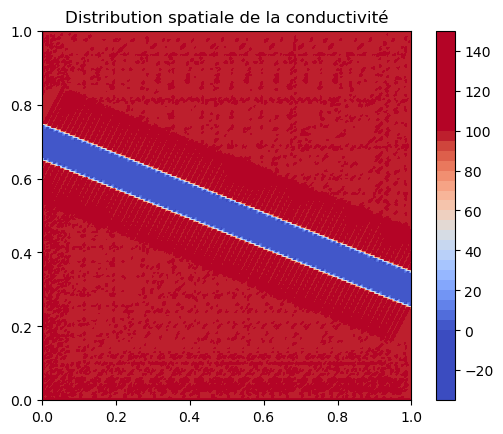
\includegraphics[height=0.65\textheight]{figures/conductivite_Kxy.png}
            
            {\small Champ de conductivité avec fracture}
        \end{column}
    \end{columns}
\end{frame}

% 5 
\begin{frame}{Conductivité paramétrée : Le défi de l'affinité}

\begin{columns}[c]
    \begin{column}{0.45\textwidth}
        Conductivité exacte (fonction indicatrice) :
        \[
        k(x,y;\mu) = D_{back} + \Delta D \cdot H(\mathcal{D}(x,y;\mu))
        \]
        
        \pause
        \vspace{0.3cm}
        \textbf{Propriétés clés :}
        \begin{itemize}
            \item Dépendance \textbf{affine} aux conductivités ($D_{back}$, $D_{frac}$).
            \item Dépendance \textbf{non affine} à la géométrie ($a$, $x_0$, $w$).
        \end{itemize}
        \vspace{0.3cm}
        \textit{Cette rupture d'affinité géométrique justifiera l'hyper-réduction.}
    \end{column}
    
    \begin{column}{0.5\textwidth}
        \centering
        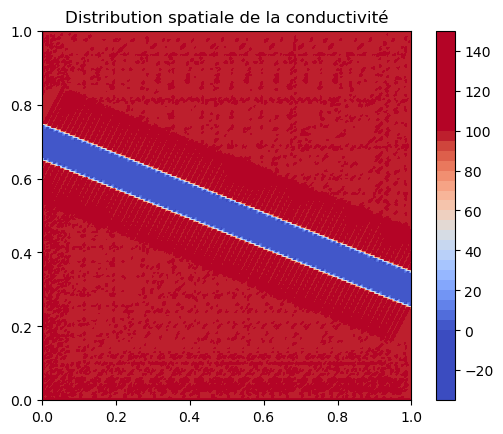
\includegraphics[height=0.65\textheight]{figures/conductivite_Kxy.png}
        
        {\small Champ de conductivité avec fracture}
    \end{column}
\end{columns}

\end{frame}

% 6 
\begin{frame}{Domaine et Conditions aux limites}

\begin{columns}[c]

\begin{column}{0.45\textwidth}
Domaine d'étude : $\Omega = [0,1]^2$

\vspace{0.3cm}
Conditions de Dirichlet imposées (scénario d'injection/drainage) :
\[
\bar{u}(x, y) = \begin{cases}
    4.0 & \text{si } (x < 0.1, y > 0.9) \\
    1.0 & \text{si } y < 0.1 \\
    0.0 & \text{ailleurs}
\end{cases}
\]
\end{column}

\begin{column}{0.50\textwidth}
\begin{center}
    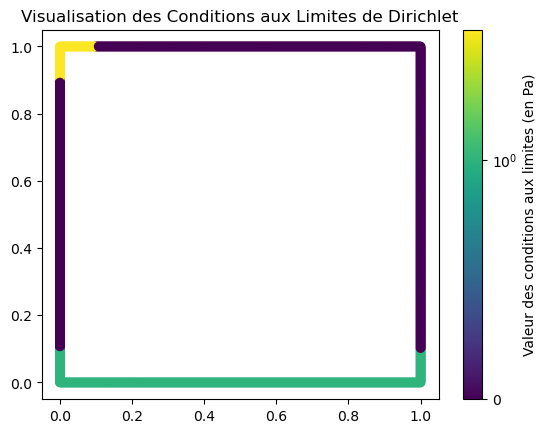
\includegraphics[width=\textwidth]{figures/conditions_limites.png}

    {\scriptsize Visualisation discrète des conditions aux limites imposées.}
\end{center}
\end{column}

\end{columns}
\end{frame}

% 7
\begin{frame}{Formulation variationnelle et Discrétisation}

\textbf{Niveau continu (après relèvement $u = u_0 + u_L$) :}
Trouver $u_0 \in H_0^1(\Omega)$ tel que :
\[
\underbrace{\int_\Omega k(\mu)\nabla u_0 \cdot \nabla v \, d\Omega}_{a(u_0, v; \mu)} = \underbrace{-\int_\Omega k(\mu)\nabla u_L \cdot \nabla v \, d\Omega}_{L(v; \mu)}
\]

\pause
\vspace{0.4cm}
\textbf{Niveau discret (Éléments Finis $\mathbb{P}2$) :}
\begin{itemize}
    \item Maillage régulier $200 \times 200 \implies \mathbf{N_{dof} = 80\,402}$.
    \item Le problème se ramène à la résolution du système linéaire complet :
\end{itemize}
\[
A(\mu)\mathbf{u}_h(\mu) = \mathbf{b}(\mu)
\]
\end{frame}

% 8 : Intégration de la solution HDM
\begin{frame}{Modèle Haute Fidélité (HDM) et goulot d'étranglement}
\begin{columns}[c]
    \begin{column}{0.45\textwidth}
        Pour chaque nouvelle configuration $\mu$, la résolution classique impose :
        \vspace{0.2cm}
        \begin{enumerate}
            \item \textbf{Assemblage :} Calcul de $A(\mu)$ sur le maillage complet ($\mathcal{O}(N_{dof})$).
            \item \textbf{Résolution :} Inversion du système creux ($\mathcal{O}(N_{dof}^{3/2})$).
        \end{enumerate}
        \vspace{0.4cm}
        Avec $80\,402$ degrés de liberté, le coût computationnel devient totalement rédhibitoire pour une exploration paramétrique.
    \end{column}
    \begin{column}{0.55\textwidth}
        \centering
        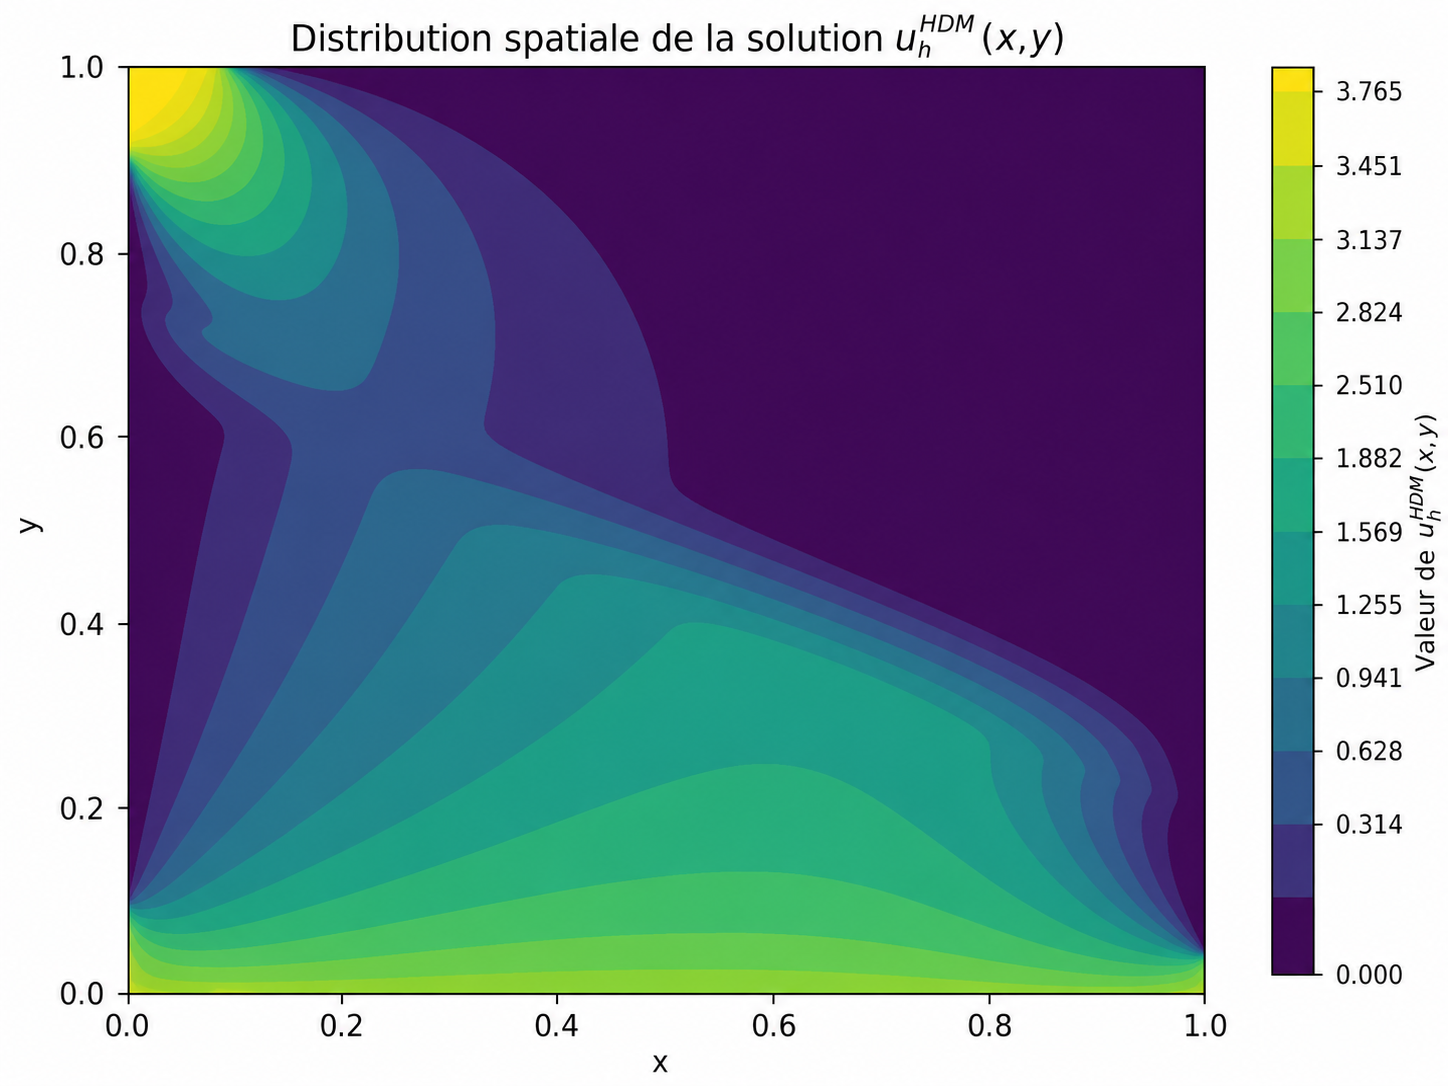
\includegraphics[width=\textwidth]{figures/graphes_projet/distribution_spatiale_solution.png}
        
        {\scriptsize Solution Haute Fidélité typique de la pression.}
    \end{column}
\end{columns}
\end{frame}

% =====================================================
\section{Réduction de modèle par POD}

% 9
\begin{frame}{L'Ensemble d'entraînement ($N_s = 200$ snapshots)}


\begin{center}
    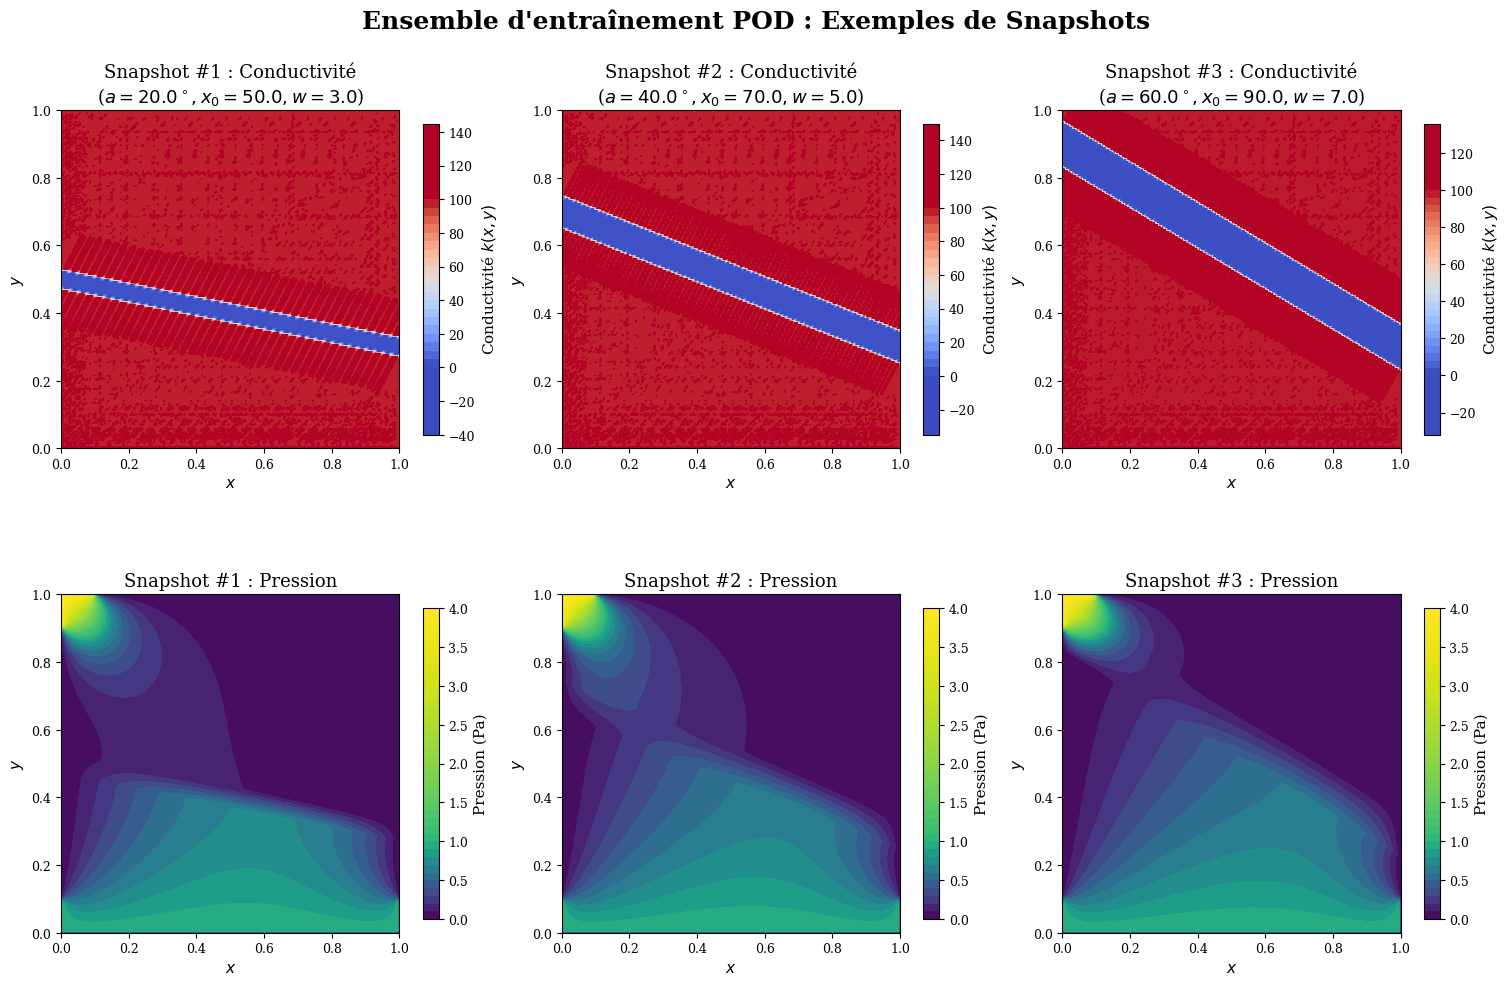
\includegraphics[width=0.6\textwidth]{figures/snapshot_1.png}

    {\scriptsize Exemples de snapshots : une grande diversité, mais une structure sous-jacente commune.}
\end{center}
\end{frame}

% 10
\begin{frame}{L'idée de la réduction par POD}

\textbf{Objectif :} Extraire une base réduite $V_r = [\varphi_1,\dots,\varphi_r]$ à partir des snapshots, avec $r \ll N_{dof}$.

\pause
\vspace{0.3cm}
La solution est alors cherchée sous la forme d'une combinaison linéaire de ces modes :
\[
\mathbf{u}_r(\mu) = V_r \mathbf{c}(\mu)
\]

\pause
\vspace{0.3cm}
\textbf{Gain théorique de la phase de résolution :}
Le système à résoudre passe d'une taille $N_{dof}$ à une taille $r$. Le coût de résolution s'effondre de $\mathcal{O}(N_{dof}^{3/2})$ à $\mathcal{O}(r^3)$.
\end{frame}

% 11 
\begin{frame}{Analyse spectrale (200 snapshots paramétriques)}
L'application de la Décomposition en Valeurs Singulières (SVD) révèle une compressibilité extrême.

\vspace{0.2cm}
\begin{columns}[c]
    \begin{column}{0.5\textwidth}
        \centering
        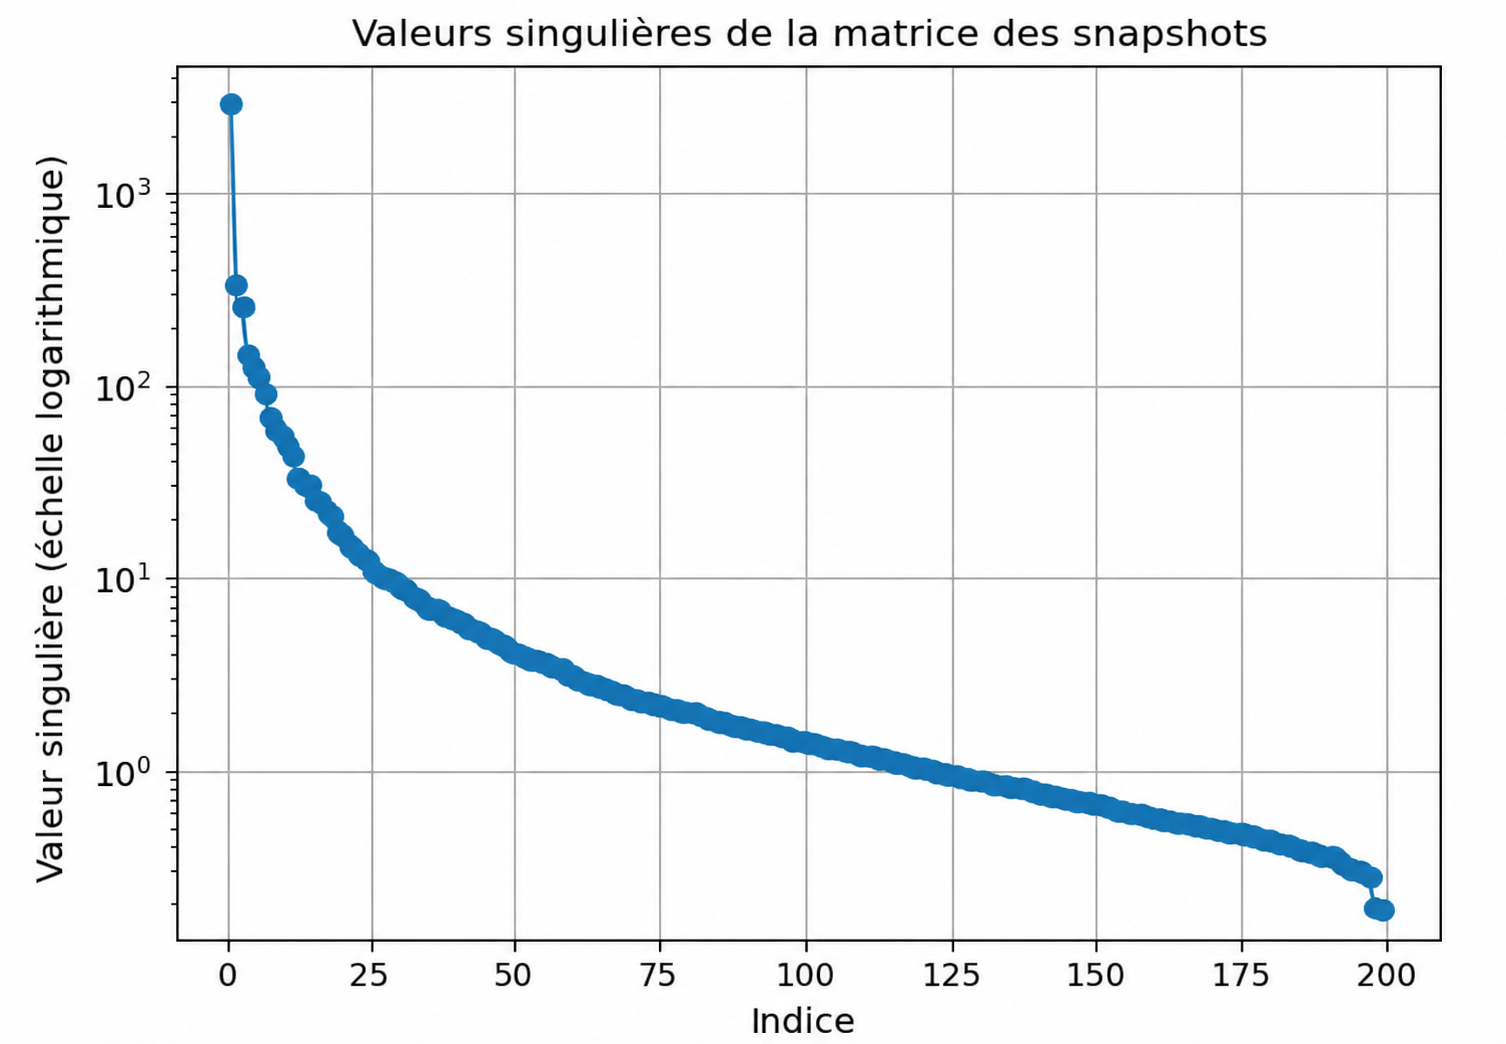
\includegraphics[width=0.95\textwidth]{figures/graphes_projet/valeurs_singulières_3.png}
    \end{column}
    \begin{column}{0.5\textwidth}
        \centering
        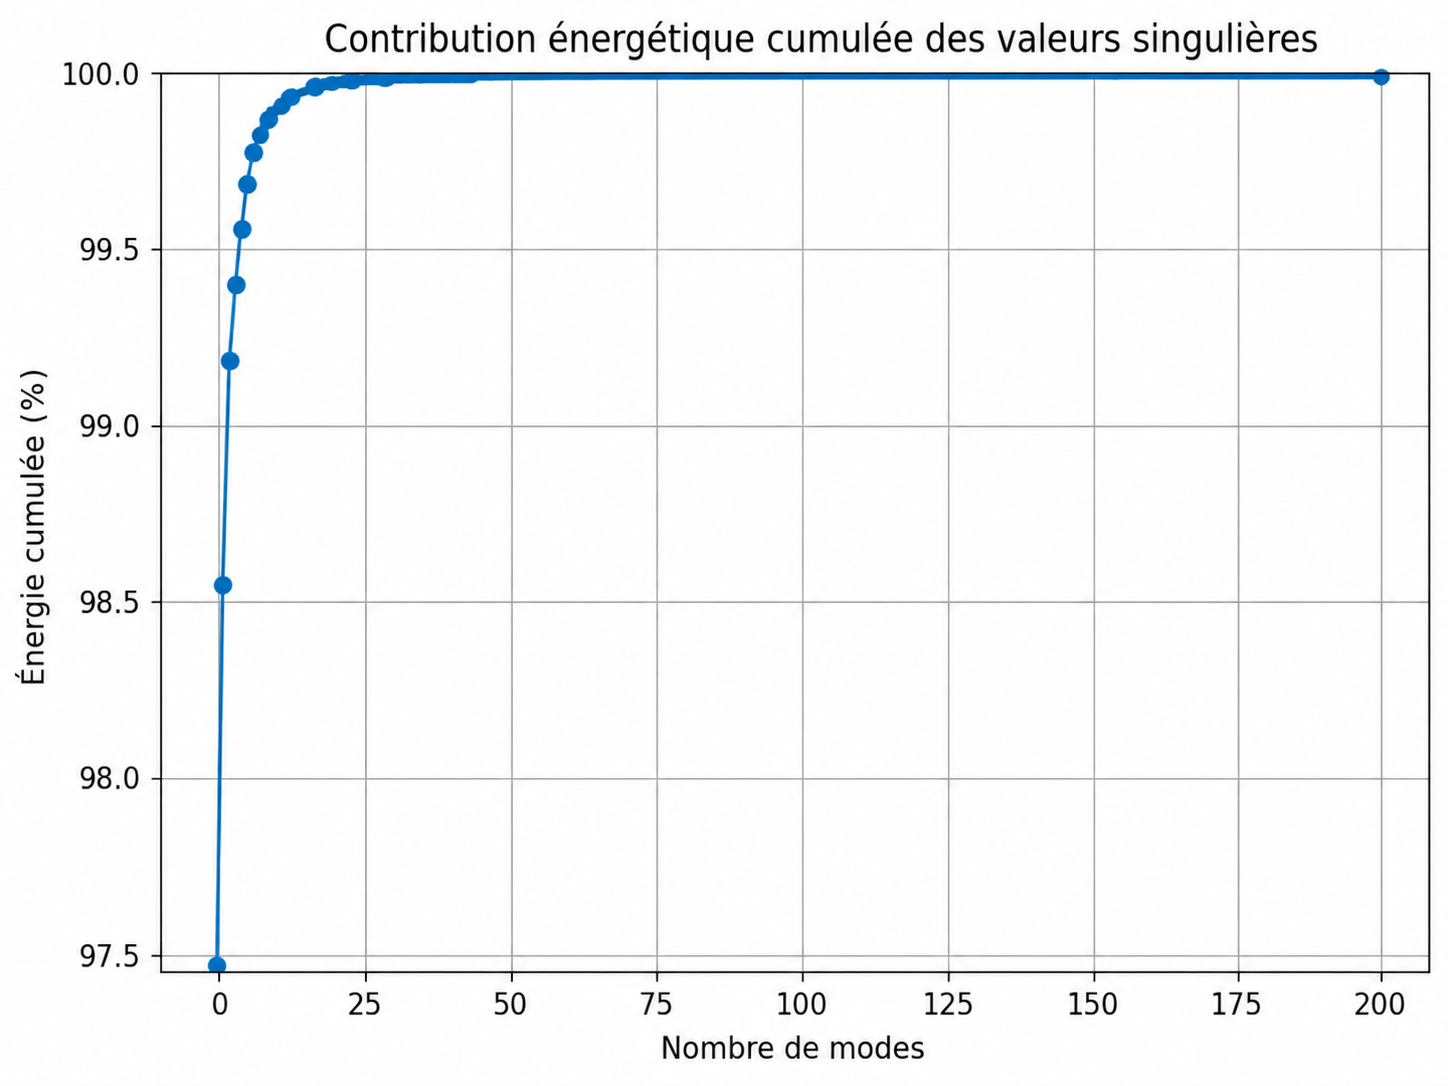
\includegraphics[width=0.95\textwidth]{figures/graphes_projet/énergie_cumulée_3.png}
    \end{column}
\end{columns}

\begin{itemize}
    \item \textbf{Résultat :} $r=20$ modes suffisent pour capturer $> 99,9\%$ de l'énergie du système.
\end{itemize}
\end{frame}

% 12
\begin{frame}{Modes POD Spatiaux}

\begin{columns}[c]
    \begin{column}{0.35\textwidth}
        \textbf{Interprétation physique :}
        \vspace{0.2cm}
        \begin{itemize}
            \item Le 1\textsuperscript{er} mode donne la tendance macroscopique imposée par le relèvement.
            \item Les modes suivants corrigent localement autour de la fracture de manière de plus en plus oscillante.
        \end{itemize}
    \end{column}
    \begin{column}{0.55\textwidth}
        \centering
        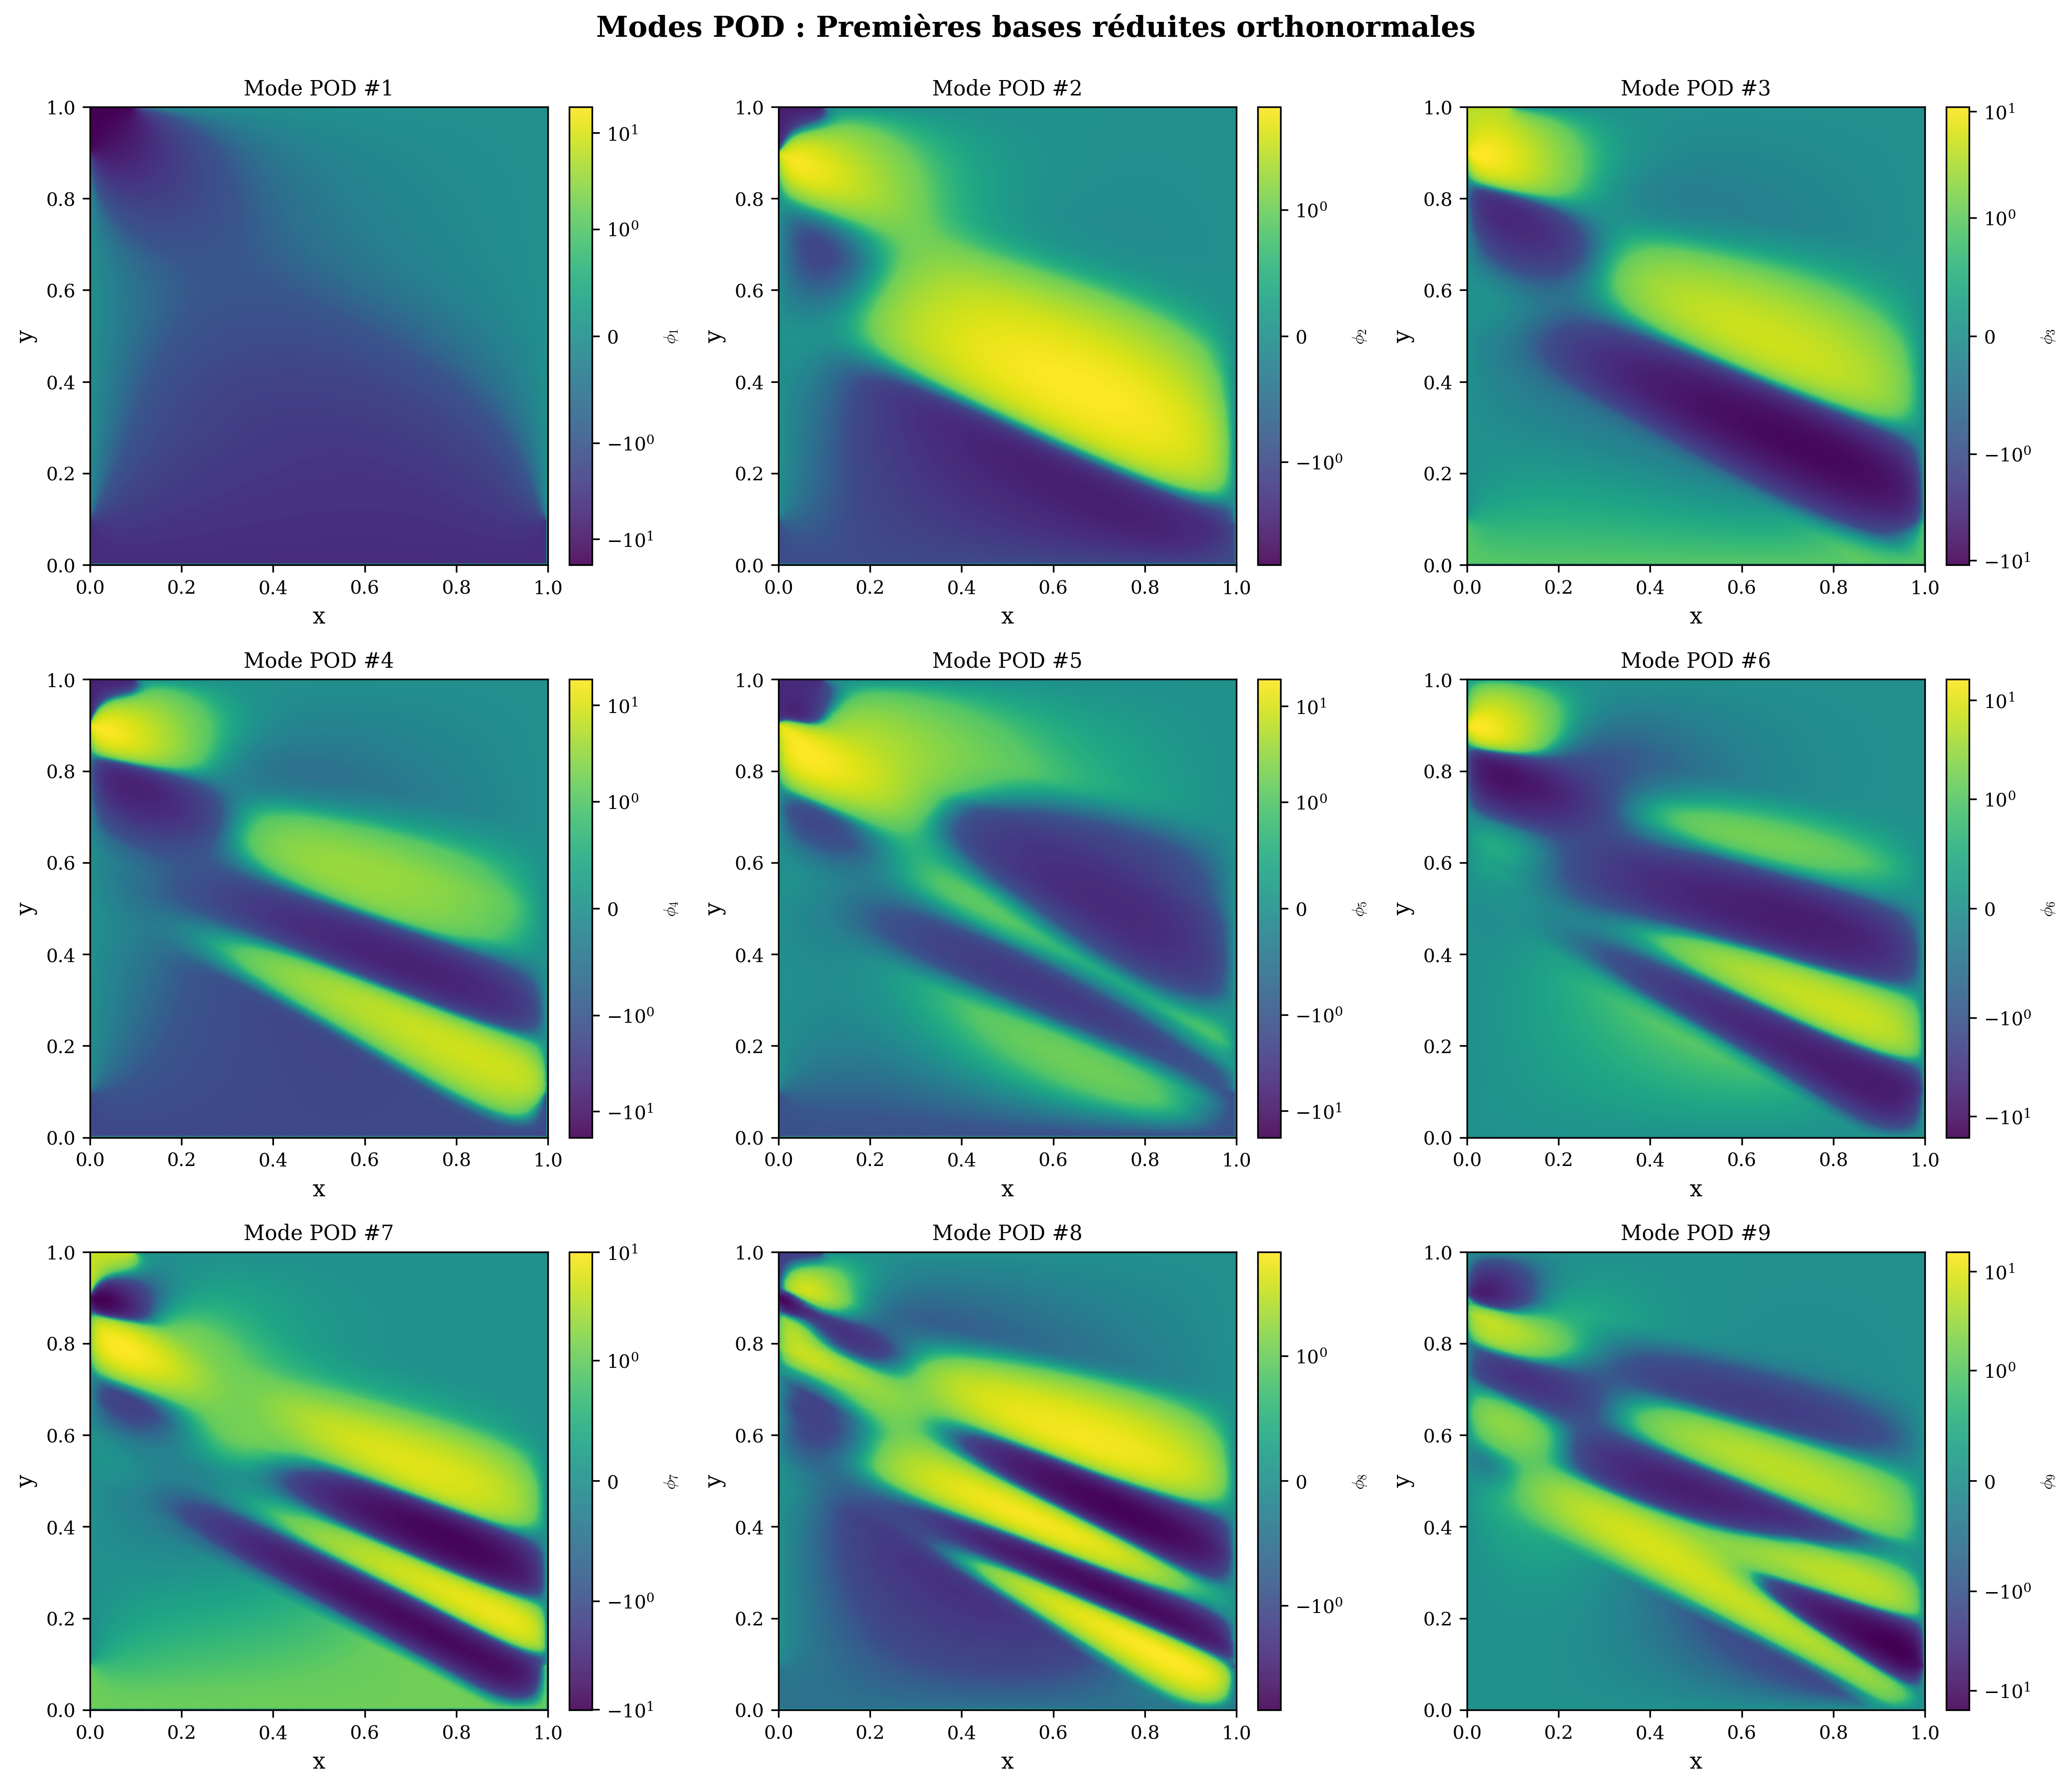
\includegraphics[width=\textwidth]{figures/03_pod_modes_9.png}
    \end{column}
\end{columns}

\end{frame}

% 13
\begin{frame}{Projection de Galerkin et Norme Énergétique}
On remplace le problème HDM par la projection de Galerkin sur $V_r$ :
\[
\underbrace{(V_r^T A(\mu)V_r)}_{A_r(\mu)} \mathbf{c}(\mu) = \underbrace{V_r^T \mathbf{b}(\mu)}_{\mathbf{b}_r(\mu)}
\]

\pause
\vspace{0.3cm}
La projection de Galerkin est optimale (projection orthogonale) pour le produit scalaire induit par la matrice $A(\mu)$. L'erreur est donc mesurée en \textbf{norme énergétique} :
\[
e_A = \frac{\|\mathbf{u}_h - \mathbf{u}_r\|_{A(\mu)}}{\|\mathbf{u}_h\|_{A(\mu)}} \quad \text{avec} \quad \|x\|_{A(\mu)} = \sqrt{x^T A(\mu) x}
\]
\end{frame}

% 14
\begin{frame}{Spectre singulier et compressibilité (Cas Affine)}

Si l'on fixe la géométrie (cas affine), la décroissance des valeurs singulières est encore plus violente (précision machine atteinte en 10 modes).

\begin{center}
    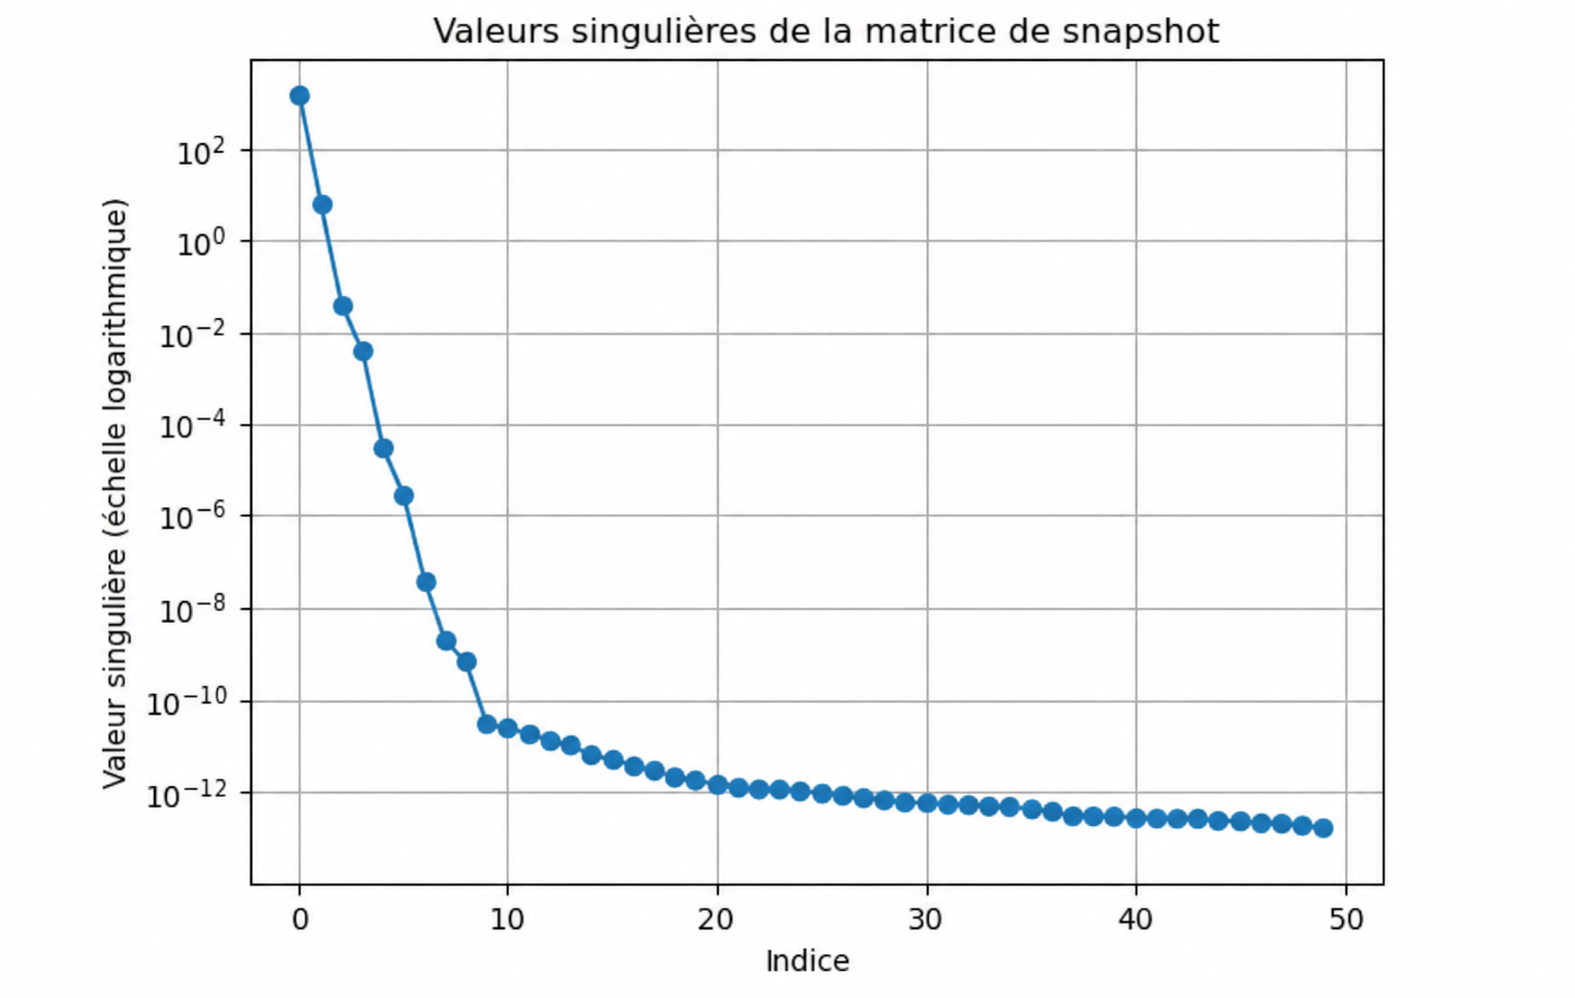
\includegraphics[height=0.6\textheight]{figures/valeurs_singulieres.png}
\end{center}
\end{frame}

% 15
\begin{frame}{Succès et Limite de la POD classique}

\begin{columns}[c]
    \begin{column}{0.45\textwidth}
        \textbf{Succès :} L'erreur chute exponentiellement. Dès $r=20$, l'erreur passe sous les $1\%$.
        
        \vspace{0.3cm}
        \textbf{Le Mur de l'Assemblage :}
        Pour construire $A_r(\mu) = V_r^T A(\mu) V_r$, il faut toujours assembler $A(\mu)$ sur le maillage complet.
        
        \[ \text{Coût Online} \sim \mathcal{O}(r^2 \mathbf{N_{dof}}) \]
    \end{column}
    \begin{column}{0.55\textwidth}
        \centering
        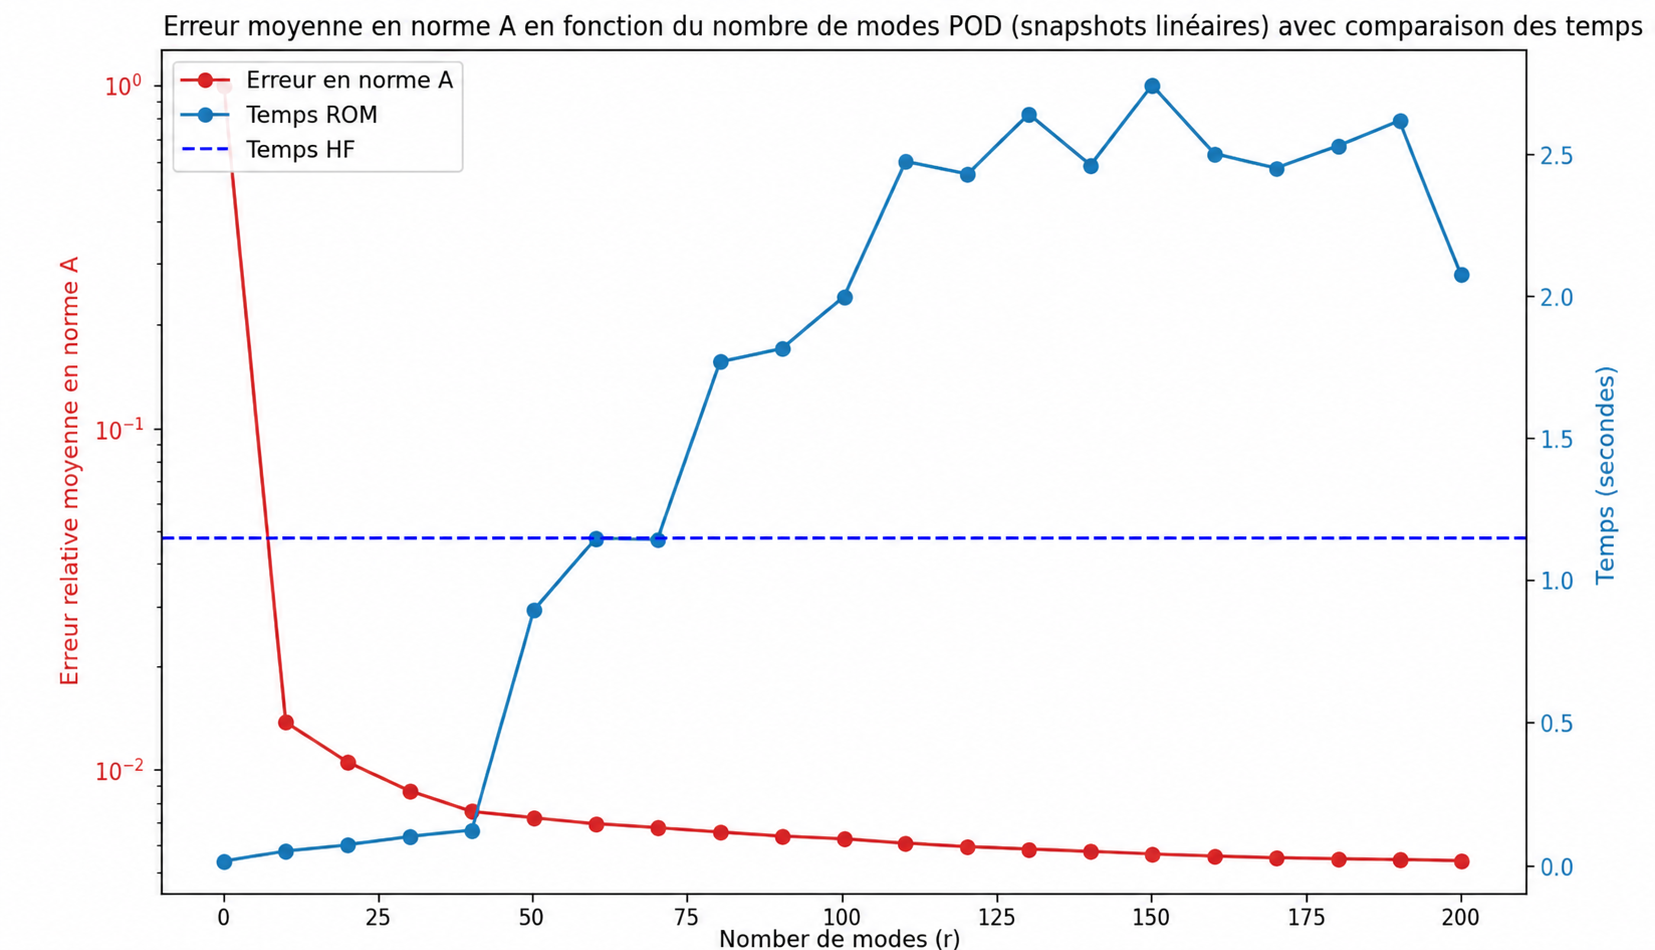
\includegraphics[width=\textwidth]{figures/erreur_normeA.png}
    \end{column}
\end{columns}
\end{frame}

% 18 : Évolution de la solution POD (Ajout)
\begin{frame}{Évolution de la reconstruction POD}
    \begin{center}
        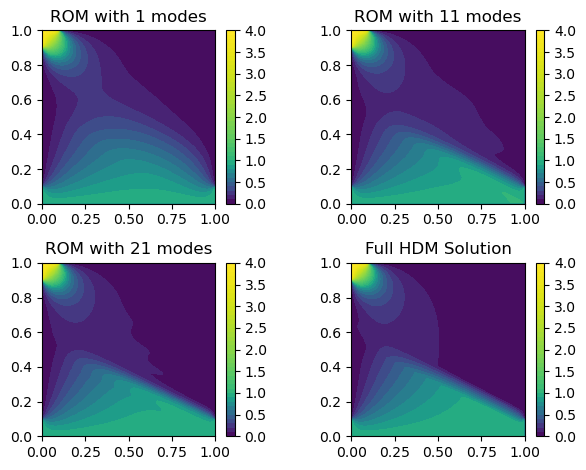
\includegraphics[width=0.55\textwidth]{figures/visu_nl.png}
    \end{center}
\end{frame}

% 16
\begin{frame}{Le remède : L'hypothèse de Décomposition Affine}

Si la conductivité s'écrit comme une somme séparable :
\[
A(\mu) = \sum_{q=1}^{Q}\theta_q(\mu)A^{(q)}
\]

\pause
\textbf{Phase Offline :} On précalcule les petites matrices $A_r^{(q)} = V_r^T A^{(q)}V_r$.

\pause
\vspace{0.2cm}
\textbf{Phase Online :} L'assemblage devient immédiat et \textbf{indépendant de $N_{dof}$} :
\[
A_r(\mu) = \sum_{q=1}^{Q}\theta_q(\mu)A_r^{(q)} \quad \longrightarrow \mathcal{O}(Q r^2)
\]

\pause
\textbf{Validation :} Dans un cas à géométrie fixée, cette séparation rend le modèle considérablement plus rapide sans aucune perte de précision.
\end{frame}

% 17
\begin{frame}{Performances dans le cas affine}
    \begin{center}
        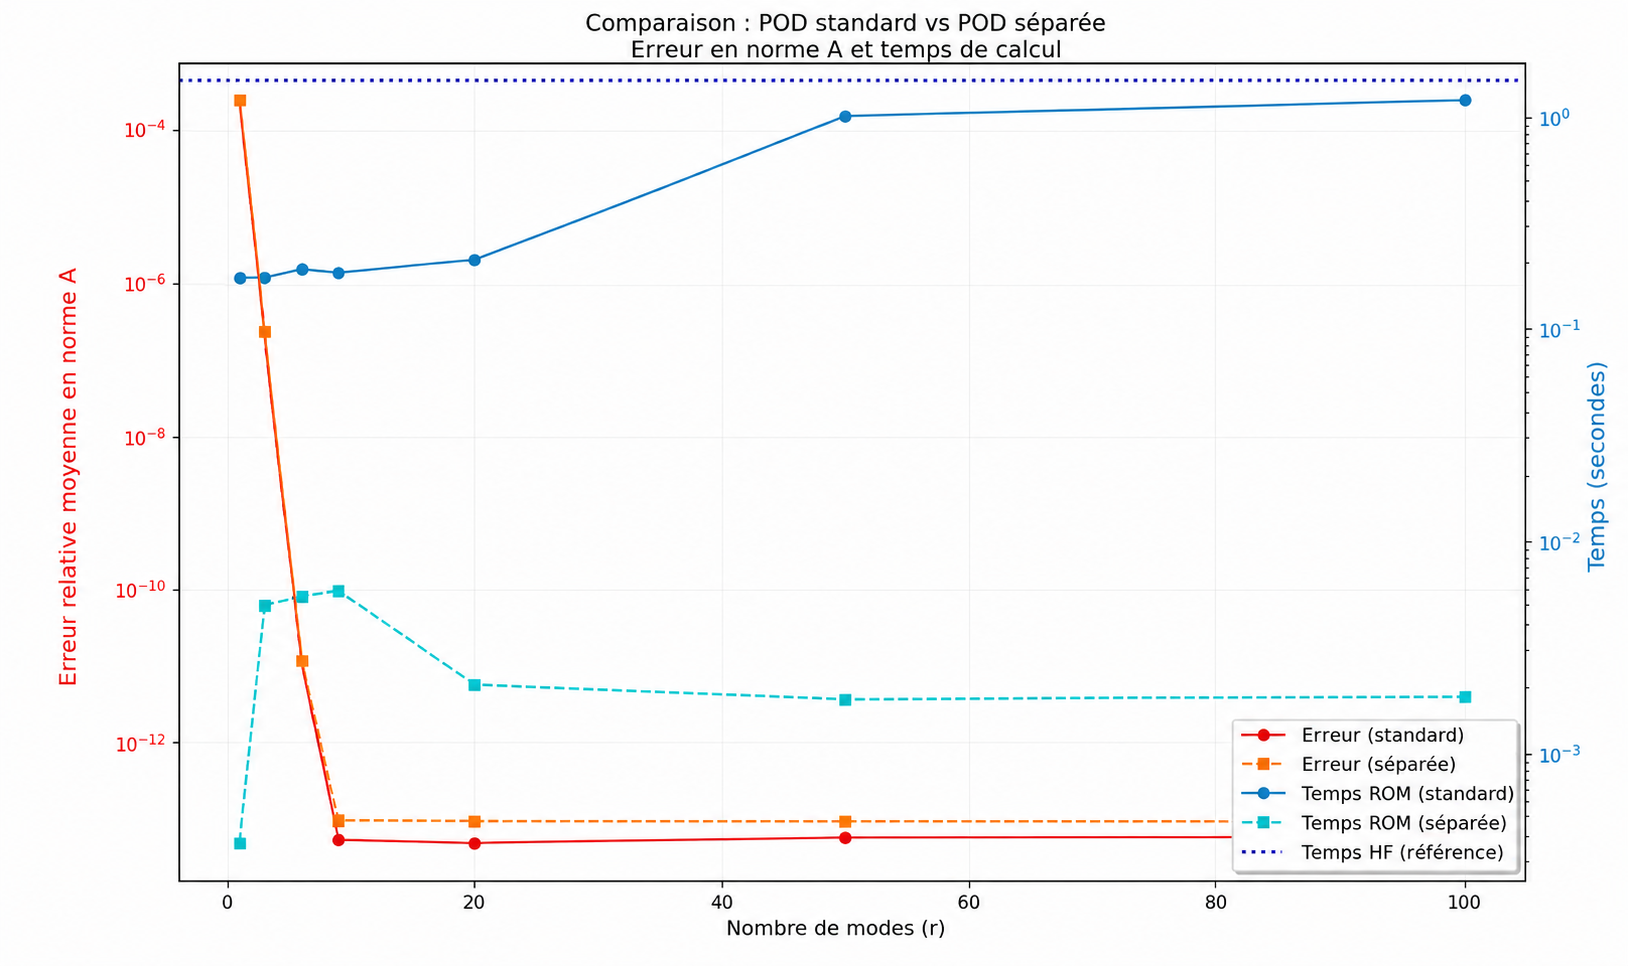
\includegraphics[height=0.7\textheight]{figures/comparaisonPOD_standard_séparée.png}
    \end{center}
\end{frame}




% =====================================================
\section{Hyper-réduction par EIM}

% 19
\begin{frame}{Pourquoi l’EIM ? La rupture géométrique}
Dès que la fracture se déplace ou s'incline, l'affinité est brisée :
\[
k(x,y;\mu) \neq \sum_{q=1}^{Q}\theta_q(\mu)k^{(q)}(x,y)
\]

\pause
\vspace{0.3cm}
L'\textbf{Empirical Interpolation Method (EIM)} vient forcer une structure affine approchée :
\[
k(x,y;\mu) \approx \sum_{m=1}^{M}\beta_m(\mu)q_m(x,y)
\]

\textbf{L'enjeu :} Calculer les coefficients $\beta_m(\mu)$ de façon très rapide, sans évaluer la fonction sur tout le maillage.
\end{frame}

% 20 : Ajout visuels modes EIM
\begin{frame}{Construction de la base EIM}
On extrait par SVD $M$ modes $q_m$ depuis $N_G = 400$ snapshots de conductivité.

\begin{center}
    \begin{tabular}{cc}
        
\includegraphics[width=0.25\textwidth]{figures/base_EIM/1.png} &
        
\includegraphics[width=0.25\textwidth]{figures/base_EIM/2.png} \\
        
\includegraphics[width=0.25\textwidth]{figures/base_EIM/3.png} &
        
\includegraphics[width=0.25\textwidth]{figures/base_EIM/4.png}
    \end{tabular}
    \end{center}
\end{frame}

% 21
\begin{frame}{Sélection des "Magic Points" : L'algorithme glouton}
L'EIM sélectionne itérativement les points d'interpolation optimaux ($t_m$) pour minimiser l'erreur d'approximation.

\vspace{0.3cm}
\begin{enumerate}
    \item<1-> \textbf{Initialisation :} On sélectionne le nœud du maillage où le premier mode $q_1$ est en valeur absolue le plus grand.
    \[ t_1 = \arg\max_x |q_1(x)| \]
    
    \item<2-> \textbf{Itération (pour $m=2 \dots M$) :}
    \begin{itemize}
        \item On interpole le mode $q_m$ sur les $m-1$ points déjà trouvés : $\mathcal{I}_{m-1}[q_m]$.
        \item On calcule l'erreur (le résidu) sur l'ensemble du maillage :
        \[ e(x) = \left| q_m(x) - \mathcal{I}_{m-1}[q_m](x) \right| \]
        \item<3-> \textbf{Sélection :} Le nouveau "magic point" $t_m$ est celui où cette erreur est \textbf{maximale}.
        \[ t_m = \arg\max_x e(x) \]
    \end{itemize}
\end{enumerate}

\vspace{0.1cm}
\uncover<4->{\textit{Résultat : on obtient une matrice d'interpolation inversible $Z_M$.}}
\end{frame}

% 22
\begin{frame}{L'interpolation EIM Finale}
Une fois les "Magic Points" identifiés, les coefficients s'obtiennent par une simple résolution de système matriciel de taille $M \times M$ :
\[
\beta(\mu) = Z_M^{-1} \, \mathbf{k}_{magic}(\mu)
\]

\vspace{0.2cm}
où $\mathbf{k}_{magic}(\mu)$ est le vecteur de conductivité évalué \textbf{uniquement} sur les $M$ magic points.

\vspace{0.4cm}
\begin{alertblock}{Gain de complexité}
L'évaluation de la conductivité passe de $\mathcal{O}(N_{dof})$ opérations à seulement $\mathcal{O}(M)$ opérations. La dépendance au maillage est totalement brisée en phase online.
\end{alertblock}

\end{frame}

% 23
\begin{frame}{Contrôle de l'erreur EIM et Discontinuité}

L'erreur d'interpolation EIM est contrôlée par la constante de Lebesgue $\Lambda_M$ et la distance au meilleur espace d'approximation (épaisseur de Kolmogorov) :
\[
\| k - \mathcal{I}_M[k] \|_{L^\infty} \leq (1 + \Lambda_M) \inf_{v \in V_M} \| k - v \|_{L^\infty}
\]

\pause
\textbf{Le drame de la discontinuité :} La fonction indicatrice physique est \textbf{discontinue}. Le terme d'approximation stagne, l'EIM échoue.

\vspace{0.1cm}
\begin{center}
    
\includegraphics[height=0.40\textheight]{figures/erreur2_final.png}
    
    {\small Sans régularisation, l'erreur EIM stagne à des niveaux inacceptables.}
\end{center}

\end{frame}

% 24
\begin{frame}{La solution : Régularisation analytique (Théorie)}

\begin{columns}[c]
    \begin{column}{0.45\textwidth}
        Remplacement de l'indicatrice stricte par une sigmoïde :
        \[ \sigma_\alpha(x)=\frac{1}{1+e^{-\alpha x}} \]
        \vspace{0.2cm}
        \begin{itemize}
            \item Garantit la régularité analytique (vitale pour la décroissance EIM).
            \item L'écart $\| H - \sigma_{\alpha} \|_{L^2}$ tend vers $0$ en $\mathcal{O}\left(\frac{1}{\sqrt{\alpha}}\right)$.
        \end{itemize}
    \end{column}
    \begin{column}{0.55\textwidth}
        \centering
        \begin{tikzpicture}
            \begin{axis}[
                axis lines = middle,
                xlabel = {$x$},
                ylabel = {Pondération},
                domain=-2:2,
                samples=150,
                ymin=-0.2, ymax=1.2,
                xmin=-2.2, xmax=2.2,
                legend pos=south east,
                grid=both,
                grid style={dashed, gray!30},
                width=\textwidth, height=0.7\textwidth,
                tick label style={font=\footnotesize, fill=white, inner sep=2pt}
            ]
                \addplot [blue, ultra thick, const plot] coordinates {(-2,0) (0,0) (0,1) (2,1)};
                \addlegendentry{$H(x)$}
                \addplot [red, thick, smooth] {1/(1 + exp(-20*x))};
                \addlegendentry{$\sigma_{20}(x)$}
            \end{axis}
        \end{tikzpicture}
    \end{column}
\end{columns}

\end{frame}




% 2ème slide : Le résultat visuel sur la conductivité
\begin{frame}{La solution : Régularisation analytique (Pratique)}
    \begin{columns}[c]
        \begin{column}{0.5\textwidth}
            \centering
            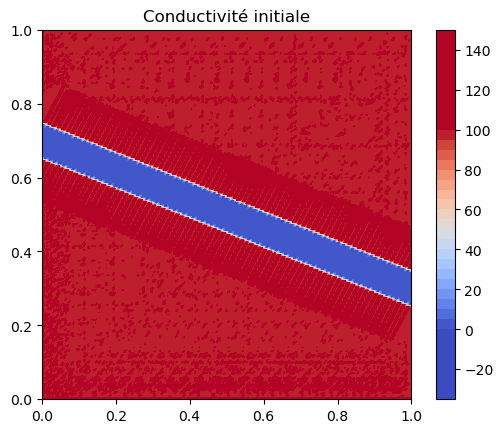
\includegraphics[width=0.85\textwidth]{figures/compare_1.png}
            
            {\small Fracture originale (Heaviside discontinue)}
        \end{column}
        \begin{column}{0.5\textwidth}
            \centering
            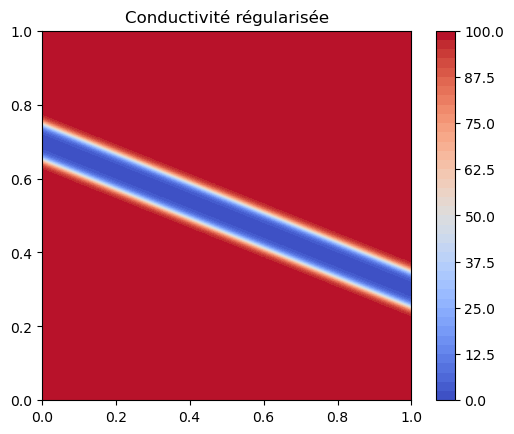
\includegraphics[width=0.85\textwidth]{figures/compare_2.png}
            
            {\small Fracture régularisée ($\alpha=150$)}
        \end{column}
    \end{columns}
    
    Ce lissage modifie l'interface physique pour la rendre continue, ce qui est l'étape indispensable pour appliquer l'algorithme EIM de manière stable.
\end{frame}

% 3ème slide : La preuve que la physique est conservée
\begin{frame}{Convergence du modèle régularisé vers la physique exacte}
    
\begin{center}
    % Image en très grand format pour bien voir l'asymptote
    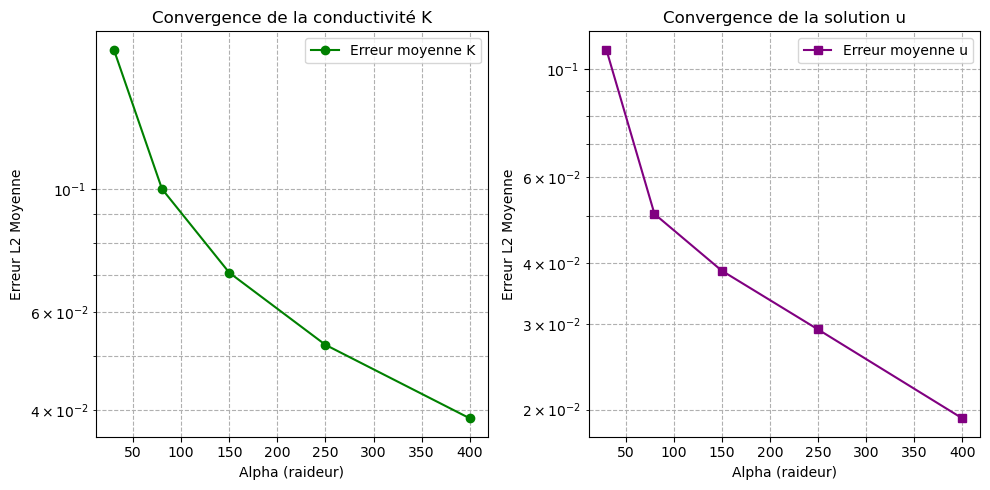
\includegraphics[height=0.75\textheight]{figures/convergence_alpha.png}
    
    \vspace{0.3cm}
    {\small L'erreur entre le modèle régularisé et le modèle exact (discontinu) tend vers zéro lorsque la raideur $\alpha$ augmente.}
\end{center}

\end{frame}

% 4ème slide : Le trade-off mathématique de l'hyper-réduction
\begin{frame}{Contrôle de l'erreur et choix du paramètre $\alpha$}

Inégalité triangulaire sur l'erreur globale d'approximation :
\[
\| k - \mathcal{I}_M[k_\alpha] \|_{L^\infty} \leq \underbrace{\| k - k_\alpha \|_{L^\infty}}_{\text{Erreur de Modèle}} + \underbrace{\| k_\alpha - \mathcal{I}_M[k_\alpha] \|_{L^\infty}}_{\text{Erreur d'Interpolation EIM}}
\]

\pause
\vspace{0.4cm}
Le choix de la raideur $\alpha$ est un \textbf{compromis strict} :
\begin{itemize}
    \item \textbf{Si $\alpha$ est trop petit :} $k_\alpha$ est trop "floue". L'erreur d'interpolation EIM converge très vite, mais l'erreur de modèle explose (on résout la mauvaise physique).
    \item \textbf{Si $\alpha$ est trop grand :} $k_\alpha$ redevient "raide". L'erreur de modèle est quasi-nulle, mais l'erreur d'interpolation EIM explose (la constante de Lebesgue domine).
\end{itemize}

\end{frame}

% 27 : Convergence EIM sur k_alpha (Ajout)
\begin{frame}{Convergence de l'EIM après régularisation}
    Avec $\alpha = 150$, la régularité est suffisante pour retrouver la convergence exponentielle prédite par la théorie.
    \begin{center}
        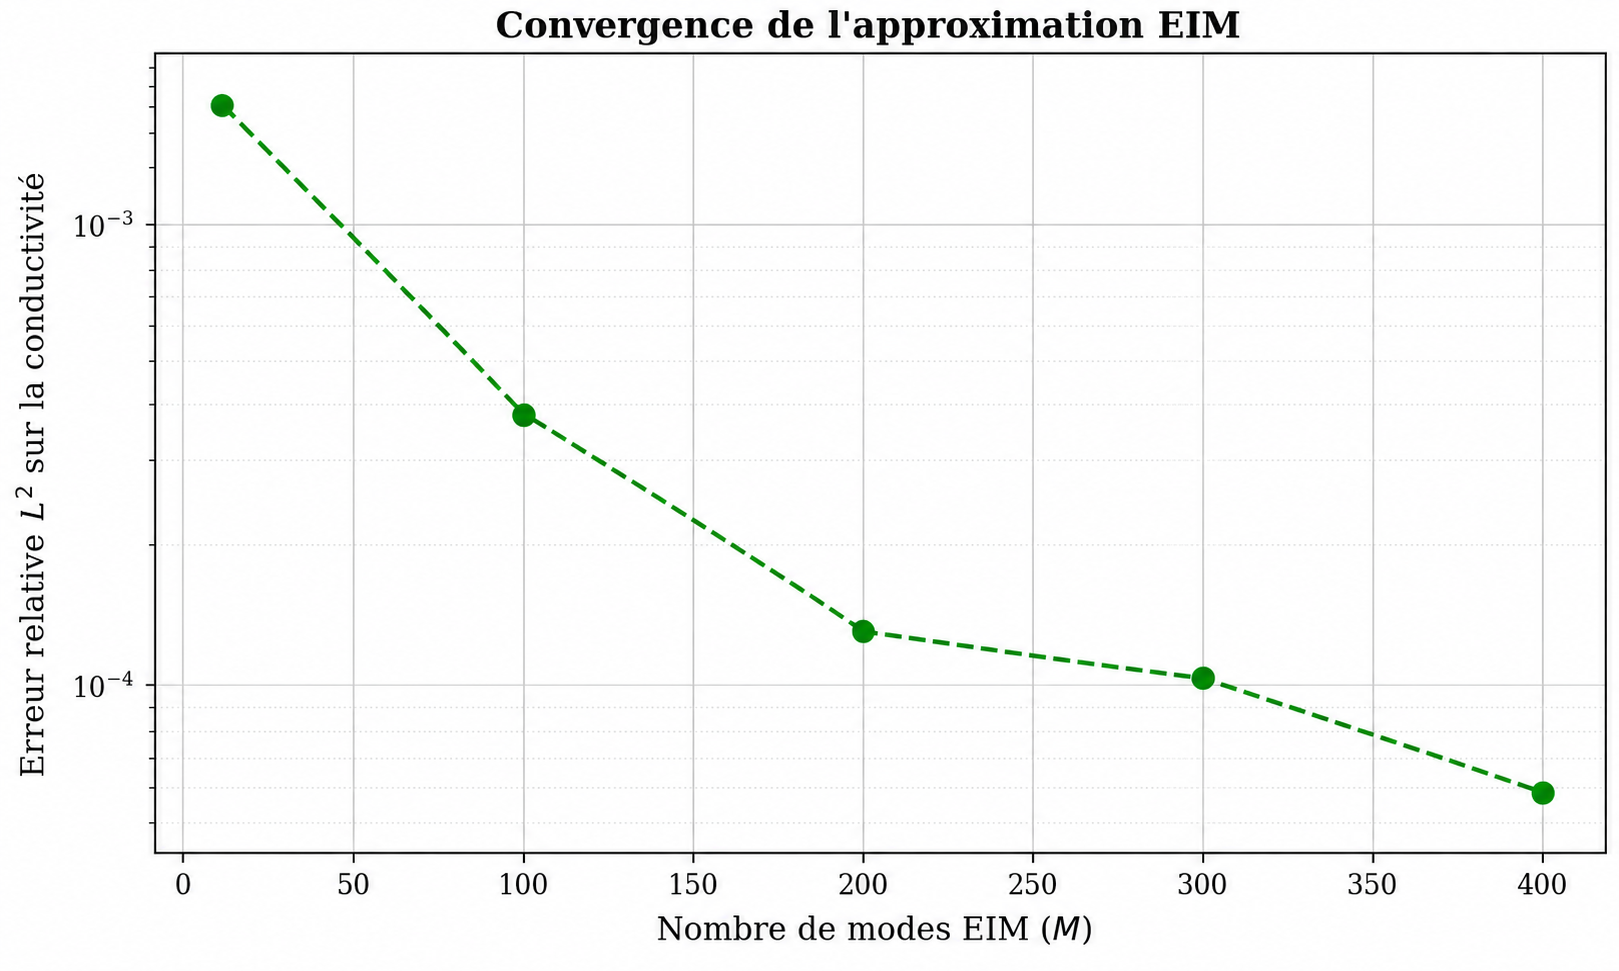
\includegraphics[height=0.65\textheight]{figures/convergence_EIM_conductivite.png}
    \end{center}
\end{frame}
% 28 : L'animation EIM propre sur une seule slide
\begin{frame}{Visualisation de l'EIM}
\begin{columns}[c]
    \begin{column}{0.5\textwidth}
        \centering
        % Le symbole % à la fin de chaque ligne est crucial : il évite les espaces
        % parasites qui pourraient faire trembler l'image.
        \includegraphics<1>[height=0.85\textheight]{figures/visu_ev_EIM/1.png}%
        \includegraphics<2>[height=0.85\textheight]{figures/visu_ev_EIM/2.png}%
        \includegraphics<3>[height=0.85\textheight]{figures/visu_ev_EIM/3.png}%
        \includegraphics<4>[height=0.85\textheight]{figures/visu_ev_EIM/4.png}%
        \includegraphics<5>[height=0.85\textheight]{figures/visu_ev_EIM/5.png}%
        \includegraphics<6>[height=0.85\textheight]{figures/visu_ev_EIM/6.png}%
        \includegraphics<7>[height=0.85\textheight]{figures/visu_ev_EIM/7.png}%
        \includegraphics<8>[height=0.85\textheight]{figures/visu_ev_EIM/8.png}%
        \includegraphics<9>[height=0.85\textheight]{figures/visu_ev_EIM/9.png}
    \end{column}
    \begin{column}{0.5\textwidth}
        \centering
        % L'image HDM n'a pas de chevron <n>, elle reste donc figée tout le temps
        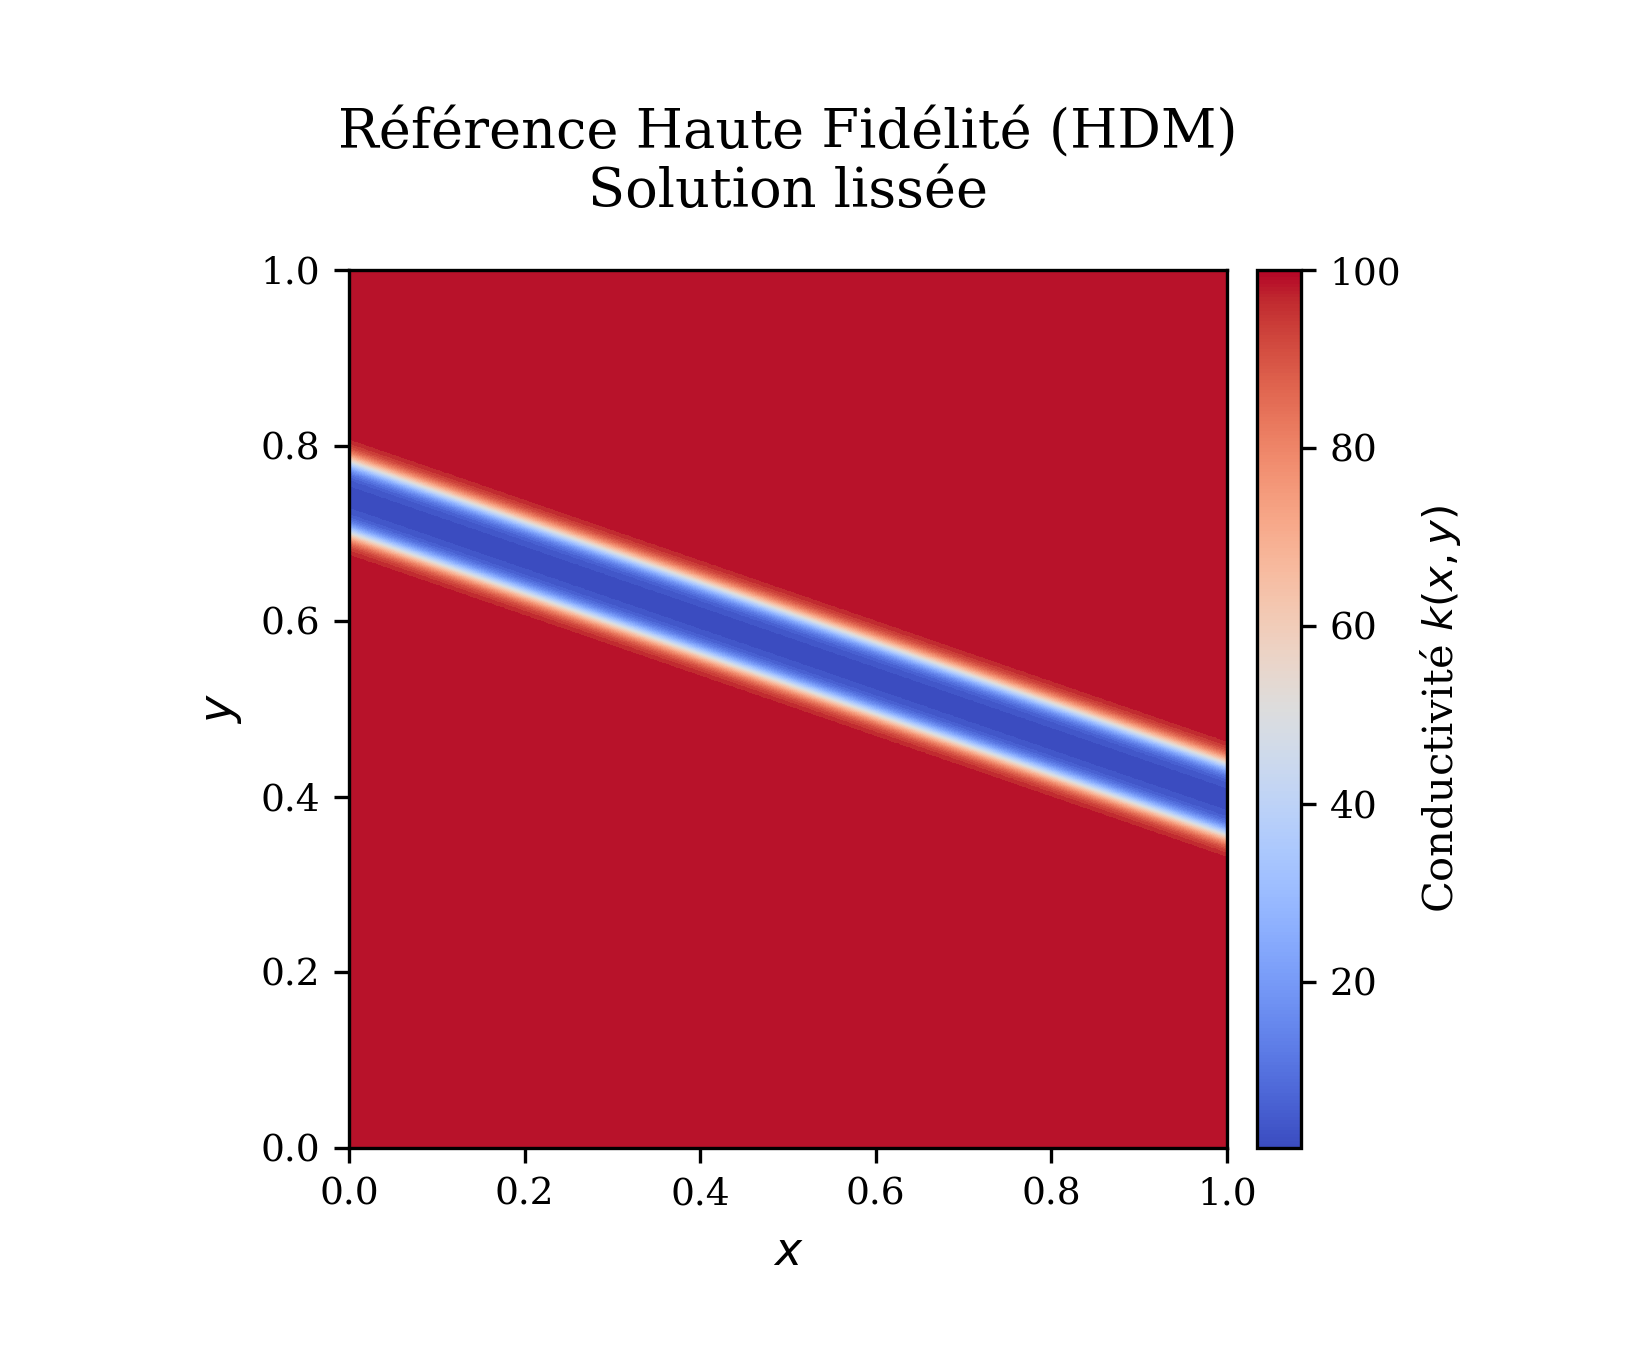
\includegraphics[height=0.85\textheight]{figures/visu_ev_EIM/HDM.png}
    \end{column}
\end{columns}
\end{frame}



% 29
\begin{frame}{Performances couplées (POD + EIM)}

\begin{columns}[c]
    \begin{column}{0.4\textwidth}
        \begin{itemize}
            \item Effondrement du temps de calcul (axe de droite, en cyan).
            \item L'erreur EIM (axe de gauche, orange) converge vers la limite théorique de la POD.
            \item L'assemblage est définitivement désolidarisé du maillage.
        \end{itemize}
    \end{column}
    \begin{column}{0.6\textwidth}
        \centering
        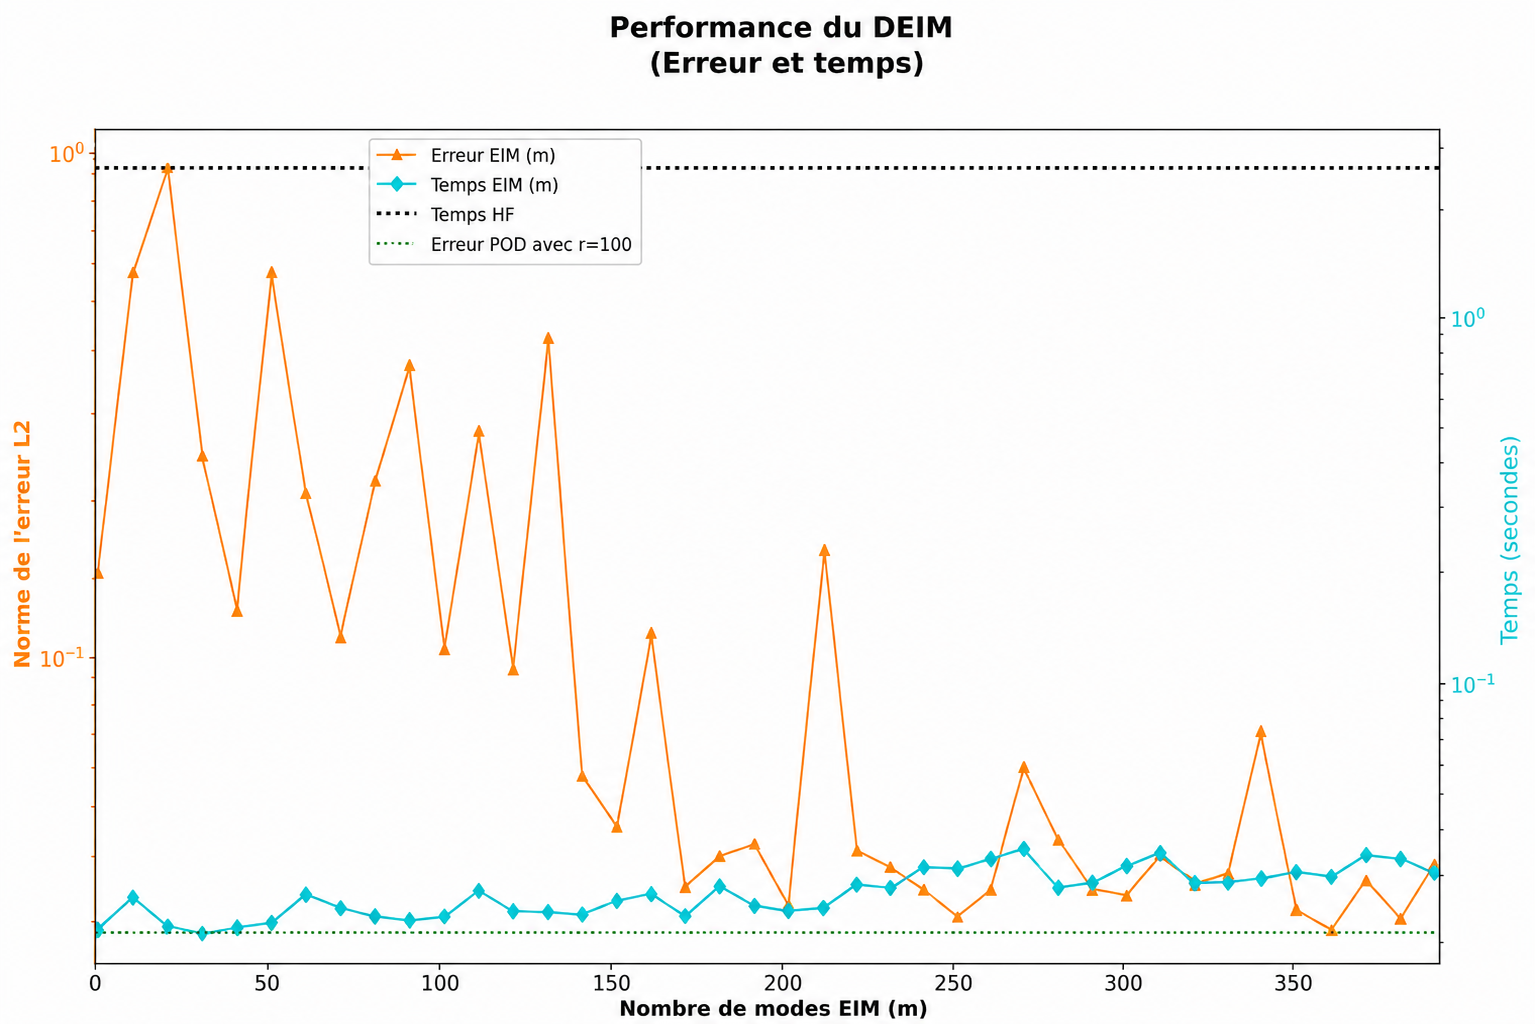
\includegraphics[width=\textwidth]{figures/perf_final_EIM.png}
    \end{column}
\end{columns}

\end{frame}

% 30
\begin{frame}{Validation Finale : Restitution de la Physique}
\begin{center}
    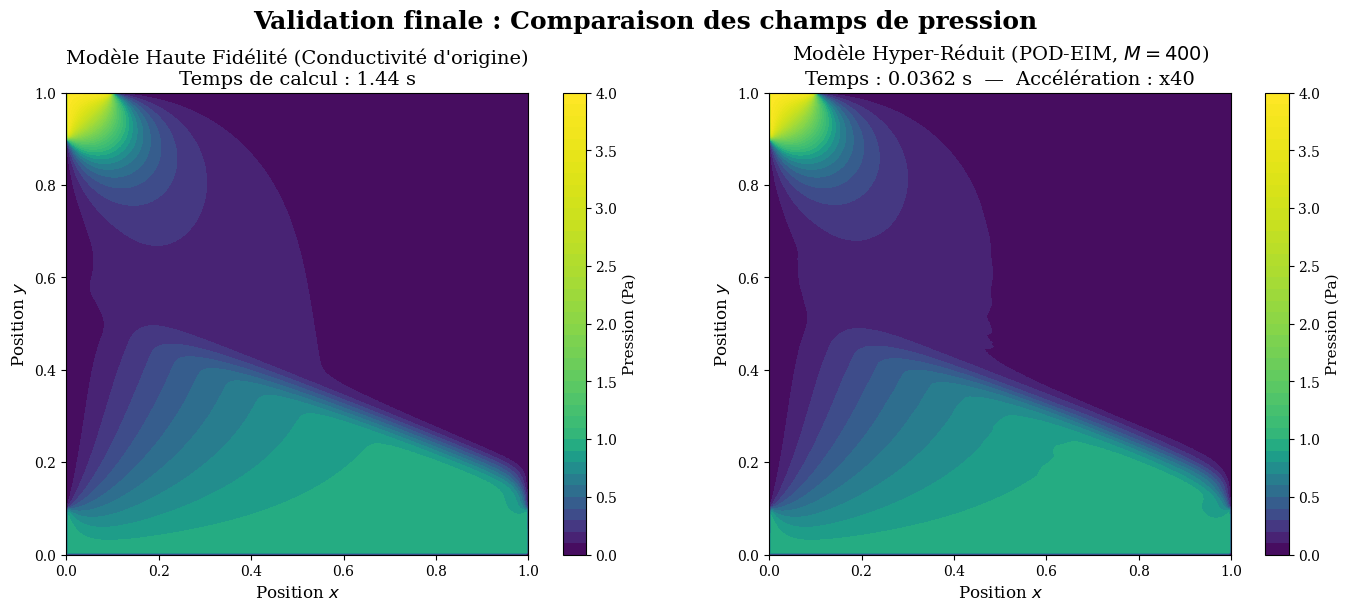
\includegraphics[height=0.65\textheight]{figures/validation_finale_pression.png}
\end{center}
\end{frame}

% =====================================================
\section{Conclusion}

% 31
\begin{frame}{Synthèse des résultats}

\textbf{Le bilan du projet :}
\begin{enumerate}
    \item \textbf{Modélisation :} Mise en place d'un solveur FEniCS robuste pour l'équation de Darcy paramétrée géométriquement ($N_{dof} > 80\,000$).
    \item \textbf{Réduction (POD) :} Identification d'une forte compressibilité spectrale permettant de reconstruire les pressions avec $\sim 20$ modes.
    \item \textbf{Hyper-Réduction (EIM) :} Contournement de la non-affinité géométrique grâce à une interpolation empirique sur des points optimaux.
\end{enumerate}

\end{frame}

% 32
\begin{frame}{Conclusion \& Perspectives}
\begin{itemize}
    \item La \textbf{régularisation analytique} s'est révélée être la clé de voûte mathématique indispensable pour appliquer l'EIM à des interfaces nettes (fractures discontinues).
    \item L'architecture Offline/Online est validée, offrant des accélérations massives du temps de résolution.
\end{itemize}

\vspace{0.5cm}
\textbf{Perspectives :}
\begin{itemize}
    \item Extension à des géométries 3D complexes.
    \item Adaptation aux problèmes dynamiques instationnaires (POD-Greedy).
    \item Développement de bornes d'erreur a posteriori certifiées.
\end{itemize}

\end{frame}

\end{document}